\documentclass{article}
\usepackage{amsmath}
\usepackage{amssymb}
\usepackage{graphicx}
\usepackage{float}
\usepackage[margin=1in]{geometry}
\usepackage{setspace}
%\onehalfspacing
\usepackage{makeidx}
\usepackage{hyperref}
\usepackage{indentfirst}
\usepackage{caption}
\usepackage{fancyhdr}
\usepackage[T1]{fontenc}
\usepackage{mdframed}
\usepackage{color}
\usepackage{xcolor}
\usepackage{enumitem}

\begin{document}
% ---- Encabezado y pie de página ----
\pagestyle{fancy}
\fancyhf{}
\fancyhead[L]{\leftmark} % Sección actual en la izquierda
\fancyhead[R]{AN1 - FaMAF} % Texto en la derecha
\renewcommand{\headrulewidth}{0.4pt} % Grosor de la línea inferior del encabezado
\fancyfoot[L]{\textbf{Ecuaciones no lineales}} % Nombre en la izquierda del pie de página
\fancyfoot[R]{\thepage} % Número de página en la derecha del pie de página
\renewcommand{\footrulewidth}{0.4pt} % Grosor de la línea superior del pie 

\section*{Método de Bisección}
\begin{mdframed}[backgroundcolor=yellow!40,shadow=true,shadowsize=2pt,roundcorner=2pt]
\begin{center}    \textbf{bisectar} = dividir en dos partes iguales. \end{center}
\end{mdframed}
\subsection*{Pasos del método}
Si $f$ es continua en $[a,b]$ y $f(a)f(b)<0$, entonces existe $c\in(a,b)$ tal que $f(c)=0$.
\begin{itemize}
    \item[1:] Se elige un intervalo [$a_0$, $b_0$] donde haya cambio de signo de la función.
    \item[2:] Se aproxima la raíz como el punto medio del intervalo
    \begin{equation*}
        x_r = \frac{a_0 + b_0}{2}
    \end{equation*}
    \item[3:] Seleccionar aquel subintervalo en que $f(x)$ cambie de signo.
    \begin{itemize}
        \item Si $f(a_0)f(x_r)<0$, entonces la raíz está en [$a_0$, $x_r$].
        \item Si $f(x_r)f(b_0)<0$, entonces la raíz está en [$x_r$, $b_0$].
    \end{itemize}
    \item[4:] Se repiten los pasos 2 y 3 hasta que se alcance la tolerancia deseada.
\end{itemize}
\subsection*{Representación gráfica}
\begin{figure}[H]
    \centering
    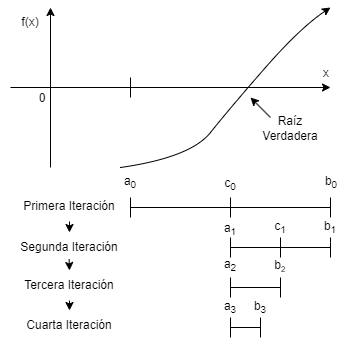
\includegraphics[width=0.5\textwidth]{bisec.png}
    \caption{Representación gráfica del método de bisección}
\end{figure}


\end{document}